\documentclass[]{article}
\usepackage{lmodern}
\usepackage{amssymb,amsmath}
\usepackage{ifxetex,ifluatex}
\usepackage{fixltx2e} % provides \textsubscript
\ifnum 0\ifxetex 1\fi\ifluatex 1\fi=0 % if pdftex
  \usepackage[T1]{fontenc}
  \usepackage[utf8]{inputenc}
\else % if luatex or xelatex
  \ifxetex
    \usepackage{mathspec}
  \else
    \usepackage{fontspec}
  \fi
  \defaultfontfeatures{Ligatures=TeX,Scale=MatchLowercase}
\fi
% use upquote if available, for straight quotes in verbatim environments
\IfFileExists{upquote.sty}{\usepackage{upquote}}{}
% use microtype if available
\IfFileExists{microtype.sty}{%
\usepackage{microtype}
\UseMicrotypeSet[protrusion]{basicmath} % disable protrusion for tt fonts
}{}
\usepackage[margin=1in]{geometry}
\usepackage{hyperref}
\hypersetup{unicode=true,
            pdftitle={R variables and data types: Introduction to R Programming},
            pdfauthor={Nicholas Ho, Richard Morris, Darya Vanichkina},
            pdfborder={0 0 0},
            breaklinks=true}
\urlstyle{same}  % don't use monospace font for urls
\usepackage{longtable,booktabs}
\usepackage{graphicx,grffile}
\makeatletter
\def\maxwidth{\ifdim\Gin@nat@width>\linewidth\linewidth\else\Gin@nat@width\fi}
\def\maxheight{\ifdim\Gin@nat@height>\textheight\textheight\else\Gin@nat@height\fi}
\makeatother
% Scale images if necessary, so that they will not overflow the page
% margins by default, and it is still possible to overwrite the defaults
% using explicit options in \includegraphics[width, height, ...]{}
\setkeys{Gin}{width=\maxwidth,height=\maxheight,keepaspectratio}
\IfFileExists{parskip.sty}{%
\usepackage{parskip}
}{% else
\setlength{\parindent}{0pt}
\setlength{\parskip}{6pt plus 2pt minus 1pt}
}
\setlength{\emergencystretch}{3em}  % prevent overfull lines
\providecommand{\tightlist}{%
  \setlength{\itemsep}{0pt}\setlength{\parskip}{0pt}}
\setcounter{secnumdepth}{0}
% Redefines (sub)paragraphs to behave more like sections
\ifx\paragraph\undefined\else
\let\oldparagraph\paragraph
\renewcommand{\paragraph}[1]{\oldparagraph{#1}\mbox{}}
\fi
\ifx\subparagraph\undefined\else
\let\oldsubparagraph\subparagraph
\renewcommand{\subparagraph}[1]{\oldsubparagraph{#1}\mbox{}}
\fi

%%% Use protect on footnotes to avoid problems with footnotes in titles
\let\rmarkdownfootnote\footnote%
\def\footnote{\protect\rmarkdownfootnote}

%%% Change title format to be more compact
\usepackage{titling}

% Create subtitle command for use in maketitle
\newcommand{\subtitle}[1]{
  \posttitle{
    \begin{center}\large#1\end{center}
    }
}

\setlength{\droptitle}{-2em}

  \title{R variables and data types: Introduction to R Programming}
    \pretitle{\vspace{\droptitle}\centering\huge}
  \posttitle{\par}
    \author{Nicholas Ho, Richard Morris, Darya Vanichkina}
    \preauthor{\centering\large\emph}
  \postauthor{\par}
    \date{}
    \predate{}\postdate{}
  

\begin{document}
\maketitle

\subsubsection{R variables and data
types}\label{r-variables-and-data-types}

First, we introduce the common variable types and data types that you'll
be working with in R. Commonly, errors involve using the wrong variable
or data type

\begin{longtable}[]{@{}lll@{}}
\toprule
\textbf{Variable type} & \textbf{Type} & \textbf{Example}\tabularnewline
\midrule
\endhead
integer & Whole numbers & 1, 100, -9\tabularnewline
numeric & Decimals & 0.1, -0.09, 234.567\tabularnewline
character & Text & ``A'', ``hello'', ``welcome''\tabularnewline
logical & Booleans & TRUE or FALSE\tabularnewline
factor & Categorical & ``green'', ``blue'', ``red'',
``purple''\tabularnewline
missing & Logical & NA\tabularnewline
empty & - & NULL\tabularnewline
\bottomrule
\end{longtable}

\begin{longtable}[]{@{}ll@{}}
\toprule
\textbf{Data type} & \textbf{Type}\tabularnewline
\midrule
\endhead
vector & 1D collection of variables of the same type\tabularnewline
matrix & 2D collection of variables of the same type\tabularnewline
data.frame & 2D collection of variables of multiple types\tabularnewline
\bottomrule
\end{longtable}

\begin{figure}
\centering
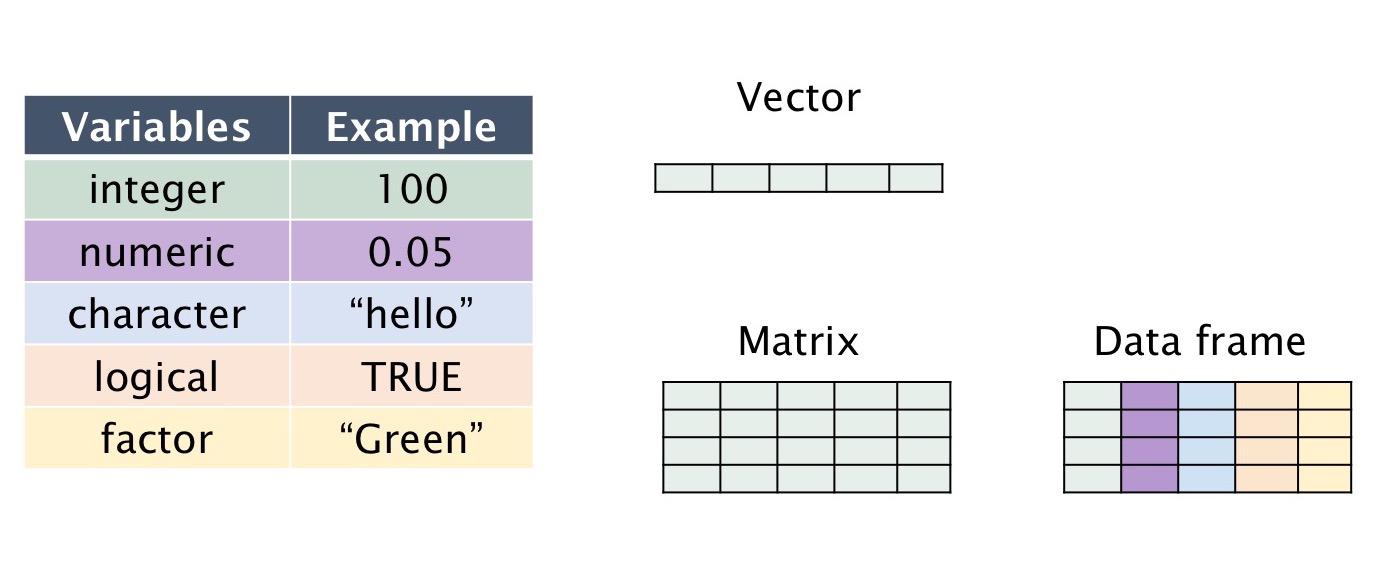
\includegraphics{Rvariablesdata.jpg}
\caption{R variable and data types}
\end{figure}

\subsection{Getting Started}\label{getting-started}

\subsubsection{Working directory}\label{working-directory}

We've created this project in a ``working directory''. To check where
this is, use:

\begin{verbatim}
getwd()
\end{verbatim}

\{: .language-r\}

\begin{verbatim}
[1] "/Users/darya/OneDrive - The University of Sydney (Staff)/Training/18_11_BMCNickHo/lessonbmc/_episodes_rmd"
\end{verbatim}

\{: .output\}

\subsubsection{Calculating things in R}\label{calculating-things-in-r}

Standard math functions work in R:

\begin{verbatim}
2+3
\end{verbatim}

\{: .language-r\}

\begin{verbatim}
[1] 5
\end{verbatim}

\{: .output\}

\begin{verbatim}
1/1000
\end{verbatim}

\{: .language-r\}

\begin{verbatim}
[1] 0.001
\end{verbatim}

\{: .output\}

\begin{verbatim}
sqrt(2)
\end{verbatim}

\{: .language-r\}

\begin{verbatim}
[1] 1.414214
\end{verbatim}

\{: .output\}

We can store values in variables. Variables are a way to both store data
and to label data.

\begin{verbatim}
myvariable <- 3
myvariable
\end{verbatim}

\{: .language-r\}

\begin{verbatim}
[1] 3
\end{verbatim}

\{: .output\}

\begin{verbatim}
myvariable = 3
myvariable
\end{verbatim}

\{: .language-r\}

\begin{verbatim}
[1] 3
\end{verbatim}

\{: .output\}

\begin{verbatim}
3 -> myvariable
myvariable
\end{verbatim}

\{: .language-r\}

\begin{verbatim}
[1] 3
\end{verbatim}

\{: .output\}

\begin{verbatim}
myvariable^2
\end{verbatim}

\{: .language-r\}

\begin{verbatim}
[1] 9
\end{verbatim}

\{: .output\} \#\# Variable and Data Types

There are several different types of data you can use in R. We'll
examine a few common ones in a little more detail.

\subsubsection{Text}\label{text}

Strings are known as ``character'' in R. Use the double quotes
\texttt{"} or single quotes \texttt{\textquotesingle{}} to wrap around
the string

\begin{verbatim}
myname <- "nick"
\end{verbatim}

\{: .language-r\}

We can use the \texttt{class()} function to see what data type it is

\begin{verbatim}
class(myname)
\end{verbatim}

\{: .language-r\}

\begin{verbatim}
[1] "character"
\end{verbatim}

\{: .output\}

\subsubsection{Numbers}\label{numbers}

Numbers have different classes. The most common two are \texttt{integer}
and \texttt{numeric}. Integers are whole numbers:

\begin{verbatim}
favourite.integer <- as.integer(8)
print(favourite.integer)
\end{verbatim}

\{: .language-r\}

\begin{verbatim}
[1] 8
\end{verbatim}

\{: .output\}

\begin{verbatim}
class(favourite.integer)
\end{verbatim}

\{: .language-r\}

\begin{verbatim}
[1] "integer"
\end{verbatim}

\{: .output\}

Numbers can be \texttt{numeric} which are decimals:

\begin{verbatim}
favourite.numeric <- as.numeric(8.8)
print(favourite.numeric)
\end{verbatim}

\{: .language-r\}

\begin{verbatim}
[1] 8.8
\end{verbatim}

\{: .output\}

\begin{verbatim}
class(favourite.numeric)
\end{verbatim}

\{: .language-r\}

\begin{verbatim}
[1] "numeric"
\end{verbatim}

\{: .output\}

\begin{verbatim}
pvalue.threshold <- 0.05
\end{verbatim}

\{: .language-r\}

\subsubsection{Logical (True/False)}\label{logical-truefalse}

We use the \texttt{==} to test for equality in R

\begin{verbatim}
class(TRUE)
\end{verbatim}

\{: .language-r\}

\begin{verbatim}
[1] "logical"
\end{verbatim}

\{: .output\}

\begin{verbatim}
favourite.numeric == 8.8
\end{verbatim}

\{: .language-r\}

\begin{verbatim}
[1] TRUE
\end{verbatim}

\{: .output\}

\begin{verbatim}
favourite.numeric == 9.9
\end{verbatim}

\{: .language-r\}

\begin{verbatim}
[1] FALSE
\end{verbatim}

\{: .output\}

\subsubsection{Vectors}\label{vectors}

We can create 1D data structures called ``vectors''.

\begin{verbatim}
1:10
\end{verbatim}

\{: .language-r\}

\begin{verbatim}
 [1]  1  2  3  4  5  6  7  8  9 10
\end{verbatim}

\{: .output\}

\begin{verbatim}
2*(1:10)
\end{verbatim}

\{: .language-r\}

\begin{verbatim}
 [1]  2  4  6  8 10 12 14 16 18 20
\end{verbatim}

\{: .output\}

\begin{verbatim}
seq(0, 10, 2)
\end{verbatim}

\{: .language-r\}

\begin{verbatim}
[1]  0  2  4  6  8 10
\end{verbatim}

\{: .output\}

We can store vectors and perform operations on them.

\begin{verbatim}
myvector <- 1:10
myvector
\end{verbatim}

\{: .language-r\}

\begin{verbatim}
 [1]  1  2  3  4  5  6  7  8  9 10
\end{verbatim}

\{: .output\}

\begin{verbatim}
2^myvector
\end{verbatim}

\{: .language-r\}

\begin{verbatim}
 [1]    2    4    8   16   32   64  128  256  512 1024
\end{verbatim}

\{: .output\}

\begin{verbatim}
b <- c(3,4,5)
b^2
\end{verbatim}

\{: .language-r\}

\begin{verbatim}
[1]  9 16 25
\end{verbatim}

\{: .output\}

\begin{verbatim}
disorders <- c("autism","ocd", "depression", "ocd", "anxiety", "autism")
disorders
\end{verbatim}

\{: .language-r\}

\begin{verbatim}
[1] "autism"     "ocd"        "depression" "ocd"        "anxiety"   
[6] "autism"    
\end{verbatim}

\{: .output\}

\subsubsection{Factors}\label{factors}

Factors store categorical data. Under the hood, factors are actually
integers that have a string label attached to each unique integer. For
example, if we have a long list of Male/Female labels for each of our
patients, this will be stored a ``row'' of zeros and ones by R.

\begin{verbatim}
disorders <- as.factor(disorders)
class(disorders)
\end{verbatim}

\{: .language-r\}

\begin{verbatim}
[1] "factor"
\end{verbatim}

\{: .output\}

How many categories are there for disorders and what are they?

\begin{verbatim}
levels(disorders)
\end{verbatim}

\{: .language-r\}

\begin{verbatim}
[1] "anxiety"    "autism"     "depression" "ocd"       
\end{verbatim}

\{: .output\}

\begin{verbatim}
nlevels(disorders)
\end{verbatim}

\{: .language-r\}

\begin{verbatim}
[1] 4
\end{verbatim}

\{: .output\}

A factor can be ordered. This makes sense in the context of a ranking
such as a survey response, e.g.~from `Strongly agree' to `Strong
disagree'.

\begin{verbatim}
responses <- c("low", "high", "medium", "low", "low", "high", "high", "medium", "medium")

myfactor <- factor(responses, levels = c("low", "medium", "high"))

myorderedfactor <- factor(responses, levels = c("low", "medium", "high"), ordered = TRUE)

levels(myfactor)
\end{verbatim}

\{: .language-r\}

\begin{verbatim}
[1] "low"    "medium" "high"  
\end{verbatim}

\{: .output\} By default, factors will be ordered in alphabetical order.

Now our factor is ordered, we can find the lowest category by using
\texttt{min()}

\begin{verbatim}
min(myfactor) #this will fail
\end{verbatim}

\{: .language-r\}

\begin{verbatim}
Error in Summary.factor(structure(c(1L, 3L, 2L, 1L, 1L, 3L, 3L, 2L, 2L: 'min' not meaningful for factors
\end{verbatim}

\{: .error\}

\begin{verbatim}
min(myorderedfactor)
\end{verbatim}

\{: .language-r\}

\begin{verbatim}
[1] low
Levels: low < medium < high
\end{verbatim}

\{: .output\}

\subsubsection{Working with data}\label{working-with-data}

A lot of the time in R, we are working with tables of data, which are
stored in a special data structure called R ``data frames''.

Commonly,

\textbf{rows} should represent instances or individual observations e.g.
\emph{data points}, \emph{patients}, \emph{events}, \emph{samples}, etc.
while

\textbf{columns} will represent different types of data associated with
each data point or instance e.g. \emph{Name}, \emph{ID},
\emph{location}, \emph{time}, \emph{value}\ldots{}

It is good practive to have a single row for every instance, and an
individual, distinct measurement in each of the columns (not multiple
measurements in one or redunant information in multiple columns). This
is called \emph{tidy data}, and makes it a lot easier to work with data
frames. It's also the source for the name ``tidyverse'', which is a
suite of packages we'll be making extensive use of in the next few weeks
to work with our data.

Here is an example data frame:

\begin{verbatim}
bmc.data <- data.frame(fname = c("Alice", "Bob", "Carol", "David"),
                       gender = as.factor(c("Female", "Male", "Female", "Male")),
                       disorder = c("autism", "anxiety", "autism", "depression"),
                       age = c(20, 45, 15, 12),
                       biomarker1 = c(5.70, 4.96, 1.37, 10.44),
                       clinicalstage = c("1b", "1a", "1a", "2"),
                       stringsAsFactors = FALSE)
\end{verbatim}

\{: .language-r\}

\subsubsection{Viewing The Data}\label{viewing-the-data}

Use the function \texttt{View()} to visually inspect the data in a new
RStudio pane:

\begin{verbatim}
View(bmc.data)
\end{verbatim}

\{: .language-r\}

How many rows and columns do we have?

\begin{verbatim}
nrow(bmc.data)
\end{verbatim}

\{: .language-r\}

\begin{verbatim}
[1] 4
\end{verbatim}

\{: .output\}

\begin{verbatim}
ncol(bmc.data)
\end{verbatim}

\{: .language-r\}

\begin{verbatim}
[1] 6
\end{verbatim}

\{: .output\}

\begin{verbatim}
dim(bmc.data)
\end{verbatim}

\{: .language-r\}

\begin{verbatim}
[1] 4 6
\end{verbatim}

\{: .output\}

\subsubsection{Accessing Subsets}\label{accessing-subsets}

Return the first N rows of your data frame

\begin{verbatim}
head(bmc.data)
\end{verbatim}

\{: .language-r\}

\begin{verbatim}
  fname gender   disorder age biomarker1 clinicalstage
1 Alice Female     autism  20       5.70            1b
2   Bob   Male    anxiety  45       4.96            1a
3 Carol Female     autism  15       1.37            1a
4 David   Male depression  12      10.44             2
\end{verbatim}

\{: .output\}

The default for the \texttt{head()} function is to show the first 6
rows. How do we know this? Type \texttt{?} infront of the function name
in your console

\begin{verbatim}
?head
\end{verbatim}

\{: .language-r\}

Return the first 3 rows of your data frame

\begin{verbatim}
head(bmc.data, n = 3)
\end{verbatim}

\{: .language-r\}

\begin{verbatim}
  fname gender disorder age biomarker1 clinicalstage
1 Alice Female   autism  20       5.70            1b
2   Bob   Male  anxiety  45       4.96            1a
3 Carol Female   autism  15       1.37            1a
\end{verbatim}

\{: .output\}

\begin{verbatim}
head(bmc.data, 3)
\end{verbatim}

\{: .language-r\}

\begin{verbatim}
  fname gender disorder age biomarker1 clinicalstage
1 Alice Female   autism  20       5.70            1b
2   Bob   Male  anxiety  45       4.96            1a
3 Carol Female   autism  15       1.37            1a
\end{verbatim}

\{: .output\}

\begin{verbatim}
bmc.data[1:3, ]
\end{verbatim}

\{: .language-r\}

\begin{verbatim}
  fname gender disorder age biomarker1 clinicalstage
1 Alice Female   autism  20       5.70            1b
2   Bob   Male  anxiety  45       4.96            1a
3 Carol Female   autism  15       1.37            1a
\end{verbatim}

\{: .output\}

\begin{verbatim}
bmc.data[c(1, 2, 3), ]
\end{verbatim}

\{: .language-r\}

\begin{verbatim}
  fname gender disorder age biomarker1 clinicalstage
1 Alice Female   autism  20       5.70            1b
2   Bob   Male  anxiety  45       4.96            1a
3 Carol Female   autism  15       1.37            1a
\end{verbatim}

\{: .output\}

\begin{verbatim}
bmc.data[c(TRUE, TRUE, TRUE, FALSE), ]
\end{verbatim}

\{: .language-r\}

\begin{verbatim}
  fname gender disorder age biomarker1 clinicalstage
1 Alice Female   autism  20       5.70            1b
2   Bob   Male  anxiety  45       4.96            1a
3 Carol Female   autism  15       1.37            1a
\end{verbatim}

\{: .output\}

As you can see, there are multiple ways to achieve the same result in R;
this is very powerful for advanced users, but can be quite confusing for
newcomers, since it's not always clear what a particular chunk of code
is doing.

Return the last 2 rows in a data set

\begin{verbatim}
tail(bmc.data, 2)
\end{verbatim}

\{: .language-r\}

\begin{verbatim}
  fname gender   disorder age biomarker1 clinicalstage
3 Carol Female     autism  15       1.37            1a
4 David   Male depression  12      10.44             2
\end{verbatim}

\{: .output\}

Return the ``age'' column in the data set

\begin{verbatim}
bmc.data$age
\end{verbatim}

\{: .language-r\}

\begin{verbatim}
[1] 20 45 15 12
\end{verbatim}

\{: .output\}

\begin{verbatim}
bmc.data[, 4]
\end{verbatim}

\{: .language-r\}

\begin{verbatim}
[1] 20 45 15 12
\end{verbatim}

\{: .output\}

\begin{verbatim}
bmc.data[, "age"]
\end{verbatim}

\{: .language-r\}

\begin{verbatim}
[1] 20 45 15 12
\end{verbatim}

\{: .output\}

Return only the first 3 rows and columns 2 and 5 of the data set

\begin{verbatim}
bmc.data[1:3, c(2,5)]
\end{verbatim}

\{: .language-r\}

\begin{verbatim}
  gender biomarker1
1 Female       5.70
2   Male       4.96
3 Female       1.37
\end{verbatim}

\{: .output\}

Return the columns named ``fname'' and ``biomarker1''

\begin{verbatim}
bmc.data[,c("fname", "biomarker1")]
\end{verbatim}

\{: .language-r\}

\begin{verbatim}
  fname biomarker1
1 Alice       5.70
2   Bob       4.96
3 Carol       1.37
4 David      10.44
\end{verbatim}

\{: .output\}

\subsubsection{Filtering the data}\label{filtering-the-data}

Return only the rows (patients) who are Female

\begin{verbatim}
bmc.data[bmc.data$gender == "Female", ]
\end{verbatim}

\{: .language-r\}

\begin{verbatim}
  fname gender disorder age biomarker1 clinicalstage
1 Alice Female   autism  20       5.70            1b
3 Carol Female   autism  15       1.37            1a
\end{verbatim}

\{: .output\}

What exactly happened here? We made a vector of \texttt{TRUE/FALSE}
statements, for each row in which this condition is true and then we
subset rows in which the index is true

\begin{verbatim}
females <- bmc.data$gender == "Female"
females
\end{verbatim}

\{: .language-r\}

\begin{verbatim}
[1]  TRUE FALSE  TRUE FALSE
\end{verbatim}

\{: .output\}

\begin{verbatim}
bmc.data[females, ]
\end{verbatim}

\{: .language-r\}

\begin{verbatim}
  fname gender disorder age biomarker1 clinicalstage
1 Alice Female   autism  20       5.70            1b
3 Carol Female   autism  15       1.37            1a
\end{verbatim}

\{: .output\}

Another way to subset the patients is with the \texttt{which()}
function. This returns the TRUE indices of a logical object.

\begin{verbatim}
females <- which(bmc.data$gender == "Female")
females
\end{verbatim}

\{: .language-r\}

\begin{verbatim}
[1] 1 3
\end{verbatim}

\{: .output\}

\begin{verbatim}
bmc.data[females, ]
\end{verbatim}

\{: .language-r\}

\begin{verbatim}
  fname gender disorder age biomarker1 clinicalstage
1 Alice Female   autism  20       5.70            1b
3 Carol Female   autism  15       1.37            1a
\end{verbatim}

\{: .output\}

\begin{verbatim}
bmc.data[which(bmc.data$gender == "Female"), ]
\end{verbatim}

\{: .language-r\}

\begin{verbatim}
  fname gender disorder age biomarker1 clinicalstage
1 Alice Female   autism  20       5.70            1b
3 Carol Female   autism  15       1.37            1a
\end{verbatim}

\{: .output\}

What if we want all patients older than 16 years of age?

\begin{verbatim}
bmc.data[bmc.data$age > 16, ]
\end{verbatim}

\{: .language-r\}

\begin{verbatim}
  fname gender disorder age biomarker1 clinicalstage
1 Alice Female   autism  20       5.70            1b
2   Bob   Male  anxiety  45       4.96            1a
\end{verbatim}

\{: .output\}

\subsubsection{Adding records}\label{adding-records}

Add a new row to the data set using the \texttt{rbind()} function:

\begin{verbatim}
new.person <- data.frame(fname = "Evelyn",
                         gender = "Female",
                         disorder = "anxiety",
                         age = 27,
                         biomarker1 = 40.8,
                         clinicalstage = "2")

bmc.data <- rbind(bmc.data, new.person)
class(bmc.data)
\end{verbatim}

\{: .language-r\}

\begin{quote}
\subsection{Section quiz}\label{section-quiz}

\begin{enumerate}
\def\labelenumi{\arabic{enumi}.}
\item
  Return those patients whose clinical stage is ``1a''
\item
  Return those patients whose biomarker1 value is less than 6.7
\item
  Return just the first name of all patients older than 16 years of age
\end{enumerate}

\{: .source\}

\begin{quote}
\subsection{Solution}\label{solution}

\begin{enumerate}
\def\labelenumi{\arabic{enumi}.}
\tightlist
\item
  Return those patients whose clinical stage is ``1a''
\end{enumerate}

\begin{verbatim}
bmc.data[bmc.data$clinicalstage == "1a",]
\end{verbatim}

\begin{enumerate}
\def\labelenumi{\arabic{enumi}.}
\setcounter{enumi}{1}
\tightlist
\item
  Return those patients whose biomarker1 value is less than 6.7
\end{enumerate}

\begin{verbatim}
bmc.data[bmc.data$biomarker1 < 6.7,]
\end{verbatim}

\begin{enumerate}
\def\labelenumi{\arabic{enumi}.}
\setcounter{enumi}{2}
\tightlist
\item
  Return just the first name of all patients older than 16 years of age
\end{enumerate}

\begin{verbatim}
bmc.data[bmc.data$age > 16,]$fname
bmc.data[bmc.data$age > 16,"fname"]
\end{verbatim}

\{: .output\} \{: .solution\} \{: .challenge\}
\end{quote}
\end{quote}


\end{document}
